
\documentclass[a4paper,12pt]{report}

% Включаем русский язык
\usepackage{latexsym}
\usepackage[warn]{mathtext}     % русские буквы буквы в формулах (с предупреждением)
\usepackage[russian]{babel}
\usepackage[utf8]{inputenc}
\usepackage[T2A]{fontenc}
\usepackage{indentfirst}        % русский стиль: отступ первого абзаца раздела
%\usepackage[nohyphen]{underscore}

% Подключаем графику
\usepackage[pdftex]{graphicx}
\pdfcompresslevel=9

\graphicspath{{./images}}

% Подключаем математические формулы
\usepackage{amsmath}
\usepackage{amsfonts}
\usepackage{amssymb}

\usepackage{cmap}               % Поиск по русским буквам в pdf

\usepackage{hyperref}

\usepackage[usenames]{color}

\newcommand{\HRule}{\rule{\linewidth}{0.5mm}}

\renewcommand{\ref}[1]{\hyperef[#1]{\ref*{#1}}}

\newcommand{\idtf}[1]{\textit{#1}}
\newcommand{\vidtf}[1]{\idtf{\_#1}}
\newcommand{\attr}[1]{\idtf{#1\_}}
\newcommand{\rel}[1]{\idtf{#1*}}

\begin{document}


\begin{titlepage}

  \begin{center}

    \vspace{6cm}

    % Title
    \HRule \\[0.4cm]
    {\huge \bfseries Руководство к выполнению расчетной работы по курсам ОИИ и ППвИС}\\[0.4cm]

    \HRule \\[1.5cm]

    % Author and supervisor
    \begin{minipage}{0.4\textwidth}
      \begin{flushright} \large
        \emph{Автор:} \\
        Д.А.~Лазуркин
      \end{flushright}
    \end{minipage}

    \vfill

    % Bottom of the page
    {\large \today}

  \end{center}

\end{titlepage}

%%% Local Variables: 
%%% mode: latex
%%% TeX-master: "main"
%%% End: 


\chapter{Построение фрагмента онтологии}
\label{cha:Onto}

Для понимания этого раздела студент должен обладать следующими
знаниями:

\begin{itemize}
\item базовые знания по теории графов
\item SC-коде и SC-алфавите
\item базовые знания о SCg-коде
\item уметь различать абсолютные и относительные понятия
\item знание правил формирования идентификаторов sc-элементов
\end{itemize}

\section{Задание}
\label{sec:Onto_task}

Во-первых, что должны сделать вы, студент, при выполнении
этого этапа расчетной работы, это выделить абсолютные и относительные
понятия своей теоретико-графовой задачи. Список понятий должен
включать не только непосредственно необходимые для решения вашей
задачи, но и те понятия, на основе которых определены непосредственно
необходимые. Таким образом, будет выделена целая иерархия понятий.

Во-вторых, для каждого понятия разработать способ представления его
экземпляров в SC-коде. Подготовить отчет в электронном варианте о
проделанной работе, который должен содержать следующее (пример отчета
приведен в разделе \ref{sec:Onto_example}):

\begin{enumerate}
\item перечень выделенных понятий со следующей информацией:
  \begin{enumerate}
  \item название понятия;
  \item абсолютное или относительное;
  \item определение на естественном языке (его стоит брать из соответствующей
    литературы);
  \item пример представления экземпляра понятия в SC-коде на
    SCg (не маленький и не большой, среднего размера). 
  \end{enumerate}
\item пять примеров на SCg входных и выходных данных для вашей
  программы (примеры нужно брать из предыдущего этапа расчетной
  работы и можно использовать сокращенную форму записи графов).
\end{enumerate}

Для рисования SCg-текстов необходимо использовать редактор KBE
(Knowledge Base Editor). Установщик и zip-архив собранной версии под
Windows можно найти в той же папке на сервере Info, откуда вы взяли
этот документ.

Мы плавно переходим к примеру выполнения 2-го этапа$\dots$

Выполненный мною пример отчета по этому этапу в docx-формате можно
найти в папке расчетной работы на сервере Info либо в конце этого
документа.  Напомню, что мы рассматриваем задачу поиска одного из
минимальных путей в неориентированном графе. Поэтому первым, чем мы
займемся, будет способ представления в SC-коде неориентированных и
ориентированных графов.


\section{Формализация понятий <<неориентированный>> и
  <<ориентированный граф>>}
\label{sec:Onto_form_undir_dir_graph}

Возьмем для рассмотрения неориентированный граф $G$:

\begin{figure}[h!]
  \centering
  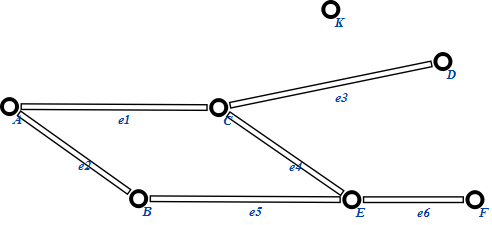
\includegraphics[scale=0.8]{2/Undirected_graph_not_scg}
  \caption{Неориентированный граф $G$ (это не SCg)}
  \label{fig:Undirected_graph_not_scg}
\end{figure}

Распишем граф $G$ классическим способом на языке теории множеств:

\begin{gather}
  G = \langle V_g,E_g \rangle; \label{eq:Graph_G_classical} \\
  V_g = \{A,B,C,E,D,F,K\}; \nonumber \\
  E_g = \{\{A,B\},\{A,C\},\{C,E\},\{C,D\},\{B,E\},\{E,F\}\}. \nonumber
\end{gather}

Теперь попробуем перевести запись, приведенную выше, в SC-код. Все
sc-конструкции я буду приводить на SCg. Для представления
неориентированного графа в SC-коде введем абсолютное понятие
\idtf{неориентированный граф} (в дальнейшем я буду использовать именно
такое форматирования для идентификаторов sc-элементов в
тексте). Теперь мы можем преобразовать запись на языке теории
множеств, задающую граф $G$, в SCg-конструкцию, которая изображена на
рис.~\ref{fig:Undirected_graph_Classical_method}.

\begin{figure}[h!]
  \centering
  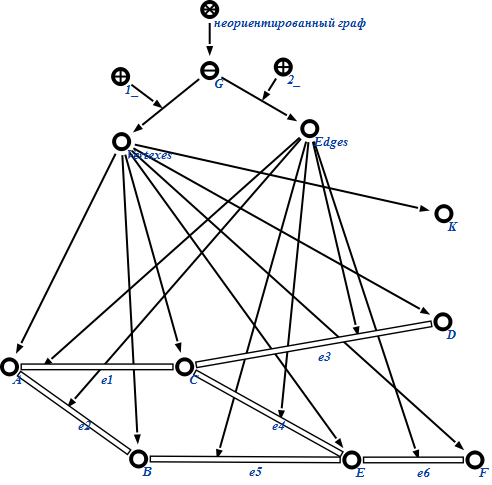
\includegraphics[scale=0.8]{2/Undirected_graph_Classical_method}
  \caption{Классический способ задания неориентированного графа $G$ на
    SCg}
  \label{fig:Undirected_graph_Classical_method}
\end{figure}

Приведенный выше способ задания графа на языке классической теории
множеств является распространённым, но мы, с использованием SC-кода,
можем найти другую форму, так как имеем возможность задавать ролевые
отношения. Поэтому введем два относительных понятия (ролевых
отношения): \idtf{вершина_} и \idtf{ребро_}. Тогда можно сформулировать,
что неориентированный граф задается множеством объектов, в котором
объект с ролью \idtf{вершина_} является вершиной графа, а объект с
ролью \idtf{ребро_} - ребром графа. На языке теории множеств,
расширенном возможностью задавать атрибуты (роли) у элементов кортежа,
граф G будет задаваться выражением~\eqref{eq:Graph_G_with_attrs}.

\begin{align}
  G &= \langle \idtf{вершина_}: A, \idtf{вершина_}: B, \idtf{вершина_}: C, \label{eq:Graph_G_with_attrs} \\
  & \idtf{вершина_}: E, \idtf{вершина_}: D, \idtf{вершина_}: F, \idtf{вершина_}: K, \nonumber \\
  & \idtf{ребро_}: \{A, B\}, \idtf{ребро_}: \{A, C\}, \idtf{ребро_}: \{C, E\}, \nonumber \\
  & \idtf{ребро_}: \{C, D\}, \idtf{ребро_}: \{B, E\},
  \idtf{ребро_}: \{E, F\} \rangle. \nonumber
\end{align}

Переведем выражение~\eqref{eq:Graph_G_with_attrs} в SCg, что показано
на рис.~\ref{fig:Undirected_graph_Main_method}.

\begin{figure}[h!]
  \centering
  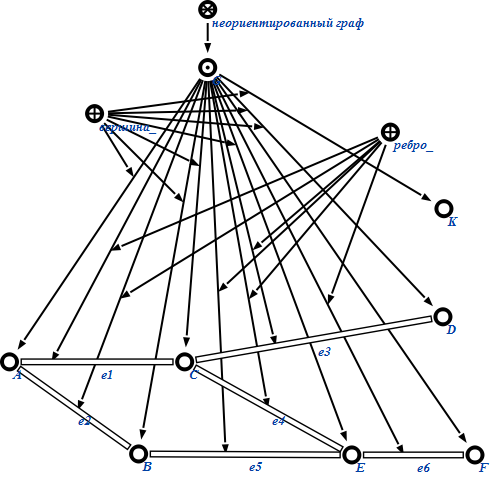
\includegraphics[scale=0.8]{2/Undirected_graph_Main_method}
  \caption{Основной для нас способ задания графа $G$ на SCg}
  \label{fig:Undirected_graph_Main_method}
\end{figure}

Для студента, знакомого с теорией множеств и SCg-языком, в
рис.~\ref{fig:Undirected_graph_Main_method} необходимо пояснить только
тип узла с идентификатором \idtf{G}. Такой тип SCg-узла используется
для обозначения sc-структуры, т.е. множества объектов, которые могут
выступать как целое. Объекты, которые входят в sc-структуру, при
совместном рассмотрении порождают некоторое новое качество. Попробуем
изучить это через сравнение множества \idtf{неориентированный граф} с
множеством \idtf{G}, которое является конкретным неориентированным
графом.

Множество \idtf{неориентированный граф} – является sc-понятием (к
слову, абсолютным), т.е. sc-множеством, все элементы которого обладают
некоторым заданным свойством. В случае sc-понятия
\idtf{неориентированный граф} его элементы должны обозначать
неориентированные графы. Предположим, в множестве
\idtf{неориентированный граф} у нас есть 5 элементов
(неориентированных графов). Добавим в это множество еще 5
неориентированных графов. При добавлении элементов мощность множества
изменилась, но качественно множество \idtf{неориентированный граф}
осталось таким же. Этот факт лаконично можно выразить следующим
образом: количество элементов множества, которое является sc-понятием,
никогда не переходит в качество.

Совсем по-другому обстоят дела с множеством \idtf{G}. Это
sc-множество, составлено из sc-элементов, которые вместе обладают
некоторой целостностью, имеющей важные свойства (они образуют
неориентированный граф только в том случае, если рассмотрены как
единое целое). Если мы добавим в множество \idtf{G} новый
элемент (вершину или ребро), то получим уже другой граф. Таким образом,
можно заключить, что количество элементов для множество \idtf{G}
переходит в качество. Множества, для которых выполняется это свойство,
являются sc-структурами.

Продолжая разговор о структурах, стоит сказать, что связки так же
являются структурами. Однако, очевидно, что неориентированный граф
\idtf{G} не только обозначает сам факт существования связи между
объектами, но и включает связки между своими собственными
элементами. Такие структуры, как граф \idtf{G} не являются связками, и
мы будем называть их одноуровневыми реляционными структурами.  Способ
представления графов в виде одноуровневых реляционных структур
используется в проекте базы знаний по теории графов технологии OSTIS
(\ostisgtlink), поэтому
ниже рассматривается только этот способ, и при выполнении расчетной
работы должен использоваться только он.

Продолжим рассмотрение того, как кодировать графы на sc-языках.
Давайте попробуем представить ориентированный граф на SCg. Преобразуем
неориентированный граф $G$ в ориентированный граф $G_d$
(рис.~\ref{fig:Directed_graph_not_scg}).

\begin{figure}[h!]
  \centering
  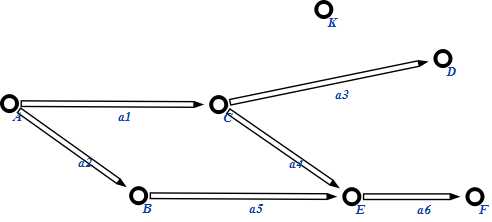
\includegraphics[scale=0.8]{2/Directed_graph_not_scg}
  \caption{Ориентированный граф $G_d$ (это не SCg)}
  \label{fig:Directed_graph_not_scg}
\end{figure}

Для представления $G_d$ на SCg введем абсолютное понятие
\idtf{ориентированный граф} и относительное понятие (ролевое
отношение) \idtf{дуга_}. С использованием этих понятий граф $G_d$ на
SCg можно представить так, как показано на
рис.~\ref{fig:Directed_graph}.

\begin{figure}[h]
  \centering
  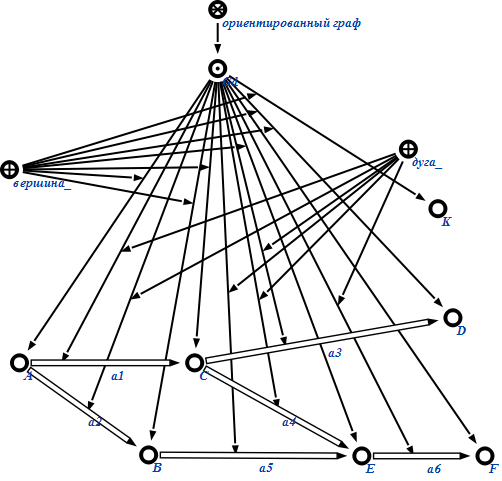
\includegraphics[scale=0.8]{2/Directed_graph}
  \caption{Ориентированный граф $G_d$ в SCg}
  \label{fig:Directed_graph}
\end{figure}

Сравните запись графа \idtf{G}
(рис.~\ref{fig:Undirected_graph_Main_method}) на SCg и графа
\idtfm{$G_d$} (рис.~\ref{fig:Directed_graph}). Разница только в
использовании:

\begin{itemize}
\item узла \idtf{ориентированный граф} вместо \idtf{неориентированный
    граф};
\item узла \idtf{дуга_} вместо \idtf{ребро_};
\item \underline{ориентированных} бинарных пар вместо
  неориентированных.
\end{itemize}

Можно заметить, что графы на SCg с использованием ролевых отношений
\idtf{вершина_} и \idtf{ребро_} получаются очень громоздкими, поэтому в
дальнейших объяснениях для представления неориентированных и
ориентированных графов мы будем использовать сокращенную запись. С
использованием сокращенной записи граф \idtf{G}, заданный на
рис.~\ref{fig:Undirected_graph_Main_method}, мы будем задавать так,
как показано на рис.~\ref{fig:Undirected_graph_Short_form}. Надеюсь:
читатель понимает, что эта запись предназначена для восприятия
человеком, а не машиной, потому что для машины является важным наличие
опущенных атрибутов.

\begin{figure}[h!]
  \centering
  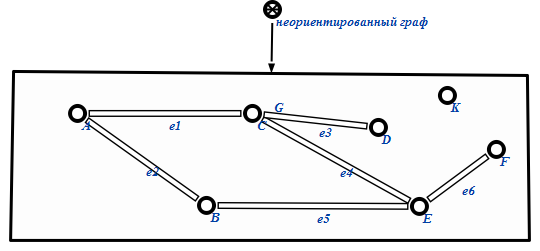
\includegraphics[scale=0.8]{2/Undirected_graph_Short_form}
  \caption{Сокращенная форма задbания графа $G$ на SCg Мы определились,}
  \label{fig:Undirected_graph_Short_form}
\end{figure}

Мы рассмотрели способ формализации с использованием семантических
сетей неориентированных и ориентированных графов. Теперь перейдем к
формализации минимального пути - второго понятия, без которого не
обойтись при решении нашей задачи.

\section{Формализация понятия <<минимальный путь>>}
\label{sec:Onto_form_min_path}

Если читатель заглянет в книгу Харарри <<Теория графов>> на страницу
26, то в начале главы <<Маршруты и связность>> он может прочитать
следующее:

\begin{quotation}
  \textbf{Маршрутом} в графе $G$ называется чередующаяся
  последовательность вершин и ребер $v_0$, $x_1$, $v_1$, $\dotsc$,
  $v_{n-1}$, $x_n$, $v_n$; эта последовательность начинается и
  кончается вершиной, и каждое ребро последовательности инцидентно
  двум вершинам, одна из которых непосредственно предшествует ему, а
  другая непосредственно следует за ним. Указанный маршрут соединяет
  вершины $v_0$ и $v_n$, и его можно обозначить $v_0$, $v_1$,
  $\dotsc$, $v_n$ (наличие ребер подразумевается). $\dots$ Маршрут
  называется \textbf{цепью}, если все его ребра различны, и
  \textbf{простой цепью} (\textbf{путем}), если все вершины (а,
  следовательно, и ребра) различны.
\end{quotation}

Таким образом, путь — это маршрут, поэтому сейчас мы будем
рассматривать именно это более общее понятие. Если разберемся с
представлением его в SC-коде, то разберемся и с более частным
понятием.

Я думаю, что для читателя очевидно следующее: маршрут – это
относительное понятие, так как конкретный маршрут существует в связи с
конкретным графом. Поэтому для представления маршрутов введем бинарное
ориентированное отношение \idtf{маршрут*}. Первым компонентом связки
этого отношения будет знак графа, а вторым знак структуры
маршрута. Пример связки приведен на
рис.~\ref{fig:Example_of_relations_Route_tuple}.

\begin{figure}[h]
  \centering
  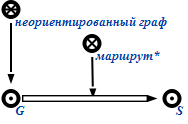
\includegraphics{2/Example_of_relations_Route_tuple}
  \caption{Пример связки отношения \idtf{маршрут*}}
  \label{fig:Example_of_relations_Route_tuple}
\end{figure}

Теперь нам необходимо выяснить из чего же состоит структура \idtf{S}
на рис.~\ref{fig:Example_of_relations_Route_tuple}. Для этого
рассмотрим в графе \idtf{G}
(рис.~\ref{fig:Undirected_graph_Short_form}) маршрут \idtf{R} между
вершинами \idtf{A} и \idtf{F}, который задается последовательностью
\idtf{A}, \idtfm{$e_2$}, \idtf{B}, \idtfm{$e_5$}, \idtf{E},
\idtfm{$e_6$}, \idtf{F} (это один из минимальных путей между \idtf{A} и
\idtf{F}). Если маршрут состоит из вершин и ребер, то его можно
представить как подграф графа, на котором задается маршрут. Посмотрите
внимательно на риc.~\ref{fig:Route_as_subgraph}.

\begin{figure}
  \centering
  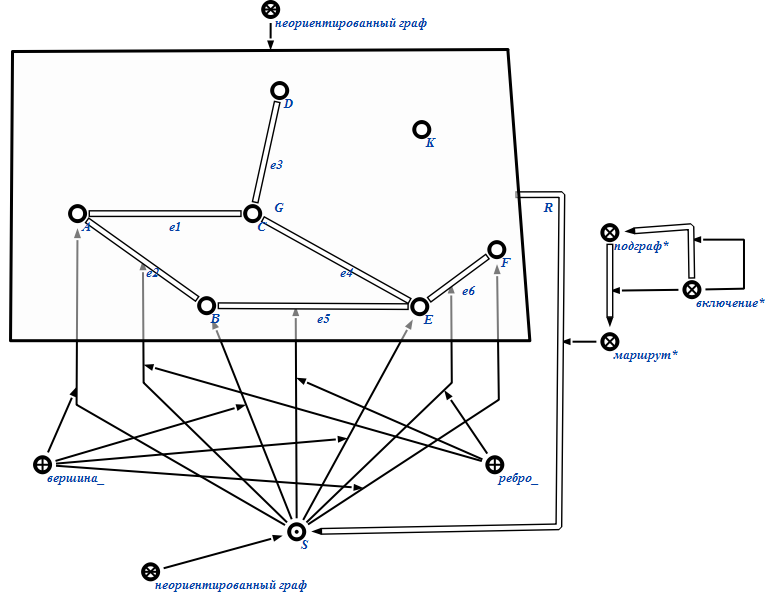
\includegraphics[scale=0.8]{2/Route_as_subgraph}
  \caption{Представление маршрута как подграфа графа \idtf{G}}
  \label{fig:Route_as_subgraph}
\end{figure}

Наверное, вы обратили внимание, что на
рис.~\ref{fig:Route_as_subgraph} появилось бинарное ориентированное
отношение \idtf{подграф*}, суть которого есть связывание одного графа
с другим графом, который является подграфом первого. А еще из
рис.~\ref{fig:Route_as_subgraph} вы можете заметить, что отношение
\idtf{включение*} включает отношение \idtf{подграф*},
т.е. \idtf{подграф*} - аналог \idtf{включения*}, но только для
графов. А наше отношение \idtf{маршрут*} является подмножеством
отношения \idtf{подграф*}. Таким образом, граф структуры \idtf{S}
является подграфом исходного графа \idtf{G}.

Возможно, вы посчитали, что на этом наш разговор о способе
представления маршрутов можно закончить, но я попрошу вас не
торопиться, а попробовать нарисовать SCg-конструкцию, которая задаст
маршрут \idtf{A}, \idtfm{$e_2$}, \idtf{B}, \idtfm{$e_5$}, \idtf{E},
\idtfm{$e_4$}, \idtf{С}, \idtfm{$e_1$}, \idtf{A}, \idtfm{$e_2$},
\idtf{B}. Ну как? Получилось? Хоть это и не путь, потому что вершины и
ребра повторяются, но это вполне допустимый маршрут. А все из-за
повторяющихся вершин и ребер. На
рис.~\ref{fig:Route_as_subgraph_problem} повторяющиеся вершины и ребра
выделены красным цветом. Поэтому мы опять переходим к поиску способа
задать структуру второго компонента связки отношения \idtf{маршрут*}
(структура \idtf{S} на
рисунке~\ref{fig:Example_of_relations_Route_tuple}).

\begin{figure}
  \centering
  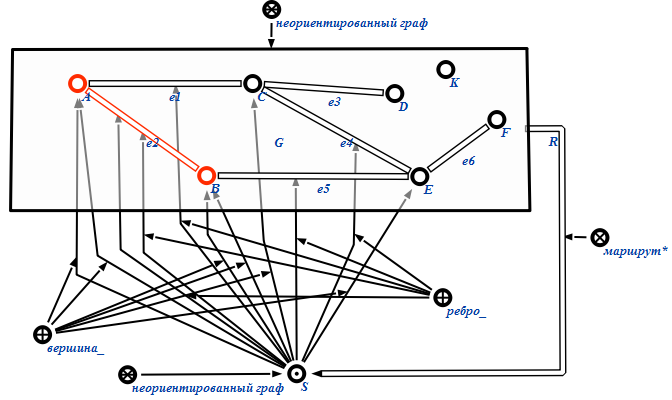
\includegraphics[scale=0.8]{2/Route_as_subgraph_problem}
  \caption{Проблема представления маршрута как подграфа графа \idtf{G}}
  \label{fig:Route_as_subgraph_problem}
\end{figure}

Вернемся к тому, что мы решили рассматривать маршрут \idtf{R} в графе
\idtf{G}. Тогда в основу нашего способа представления мы положили, что
маршрут состоит из вершин и ребер и он есть подграф графа, на котором
задается. Может быть, слабость этого подхода была в том, что мы не
рассматривали маршрут как последовательность вершин и ребер, т.е. мы
не задали порядок? Давайте попробуем задать последовательность
элементов маршрута.

Как мы можем задать последовательность? Если без введения лишних
понятий, то, например, при помощи ориентированного графа. Вершинами
такого графа будут элементы последовательности, а дуги будут задавать
отношение предыдущий/следующий. Первый элемент последовательности
специально указывать не будем, потому что первым элементом является
вершина, в которую нет входящих дуг. Последним элементом
последовательности будет вершина, из которой нет исходящих дуг. Этот
способ представления маршрута \idtf{R} показан на
рис.~\ref{fig:Route_as_sequence} (\textcolor{blue}{синим цветом}
выделены элементы маршрута, а \textcolor{green}{зеленым} - связки
следующий/предыдущий).

\begin{figure}
  \centering
  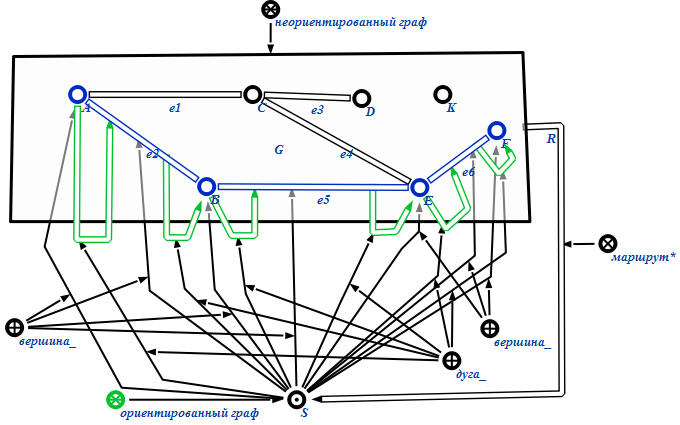
\includegraphics[scale=0.8]{2/Route_as_sequence}
  \caption{Представление маршрута через ориентированный граф последовательности}
  \label{fig:Route_as_sequence}
\end{figure}

Но, даже используя новый способ представления, мы не сможем задать
маршрут, который не является цепью или простой цепью (путем). Новый
способ представления все равно ограничен. Предлагаю вам увидеть это
самостоятельно, представив маршрут с повторяющимися вершинами и
ребрами. Поэтому продолжим наш поиск.

Давайте еще раз взглянем на определение маршрута из <<Теории графов>>:

\begin{quotation}
  \textbf{Маршрутом} в графе $G$ называется чередующаяся
  последовательность вершин и ребер $v_0$, $x_1$, $v_1$, $\dotsc$, $v_{n-1}$,
  $x_n$, $v_n$;
\end{quotation}

В нем сказано, что маршрут состоит из вершин и ребер. Но, быть может,
это не совсем так? Мы нашли два ограниченных способа для представления
маршрута, пользуясь буквально этим определением, а задачу еще не
решили. Может быть, стоит сказать, что маршрут состоит не из
последовательности вершин и ребер, а из последовательности посещений
вершин и ребер. Давайте попробуем использовать именно такую точку
зрения. Тогда мы можем преобразовать ориентированный граф
последовательности \idtf{S} из рис.~\ref{fig:Route_as_sequence} в
ориентированный граф посещений \idtf{S} на
рис.~\ref{fig:Route_as_correspondence_Incomplete}. Вершина графа
\idtf{S} на рис.~\ref{fig:Route_as_correspondence_Incomplete}
обозначает посещение вершины графа \idtf{G}, а дуга графа \idtf{S} –
посещение ребра графа \idtf{G}.

\begin{figure}[h!]
  \centering
  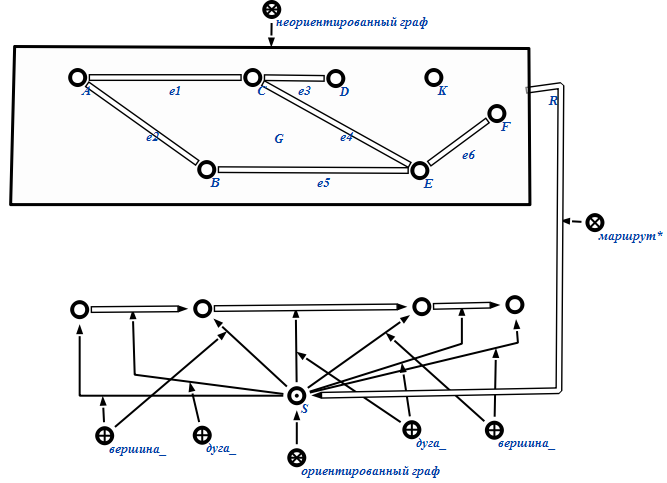
\includegraphics[scale=0.8]{2/Route_as_correspondence_Incomplete}
  \caption{Представление структуры \idtf{S} маршрута \idtf{R} как
    ориентированного графа посещений}
  \label{fig:Route_as_correspondence_Incomplete}
\end{figure}

На рис.~\ref{fig:Route_as_correspondence_Incomplete} не хватает только
связей между элементами посещения из графа $S$ и посещенными
элементами из графа $G$. Для того, чтобы мы могли закончить
конструкцию рис.~\ref{fig:Route_as_correspondence_Incomplete}, вам
надо вспомнить, что такое соответствие между двумя множествами, а,
если вы этого не знаете, то устранить пробел в вашем образовании. А
тем временем мы введем относительное понятие (тернарное отношение)
\idtf{соответствие*}, связка которого включает следующие три
компонента (пример связки на
рис.~\ref{fig:Relation_Correspondence_example}):

\begin{enumerate}
\item множество, которое является областью определения соответствия
  (множество \idtf{X}).
\item множество, которое является областью значений соответствия
  (множество \idtf{Y}).
\item бинарное ориентированное отношение, которое устанавливает
  соответствие между элементом из области определения и элементом из
  области значения (отношение \idtf{Cr*}).
\end{enumerate}

\begin{figure}[h!]
  \centering
  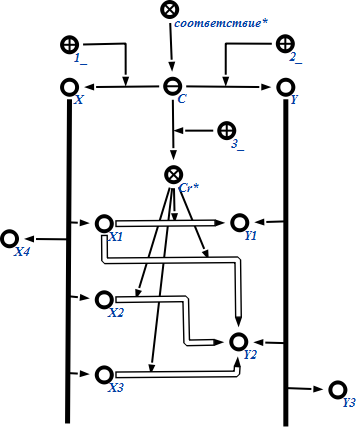
\includegraphics[scale=0.8]{2/Relation_Correspondence_example}
  \caption{Пример связки C отношения \idtf{соответствие*} между
    множествами $X$ и $Y$}
  \label{fig:Relation_Correspondence_example}
\end{figure}

Мы можем рассматривать маршрут \idtf{R} как всюду определенное,
функциональное соответствие между ориентированным графом (структурой
маршрута) \idtf{S} и неориентированным исходным графом \idtf{G}.
Тогда на основе
рис.~\ref{fig:Route_as_correspondence_Incomplete}~и~\ref{fig:Relation_Correspondence_example}
построим окончательный вариант представления маршрута \idtf{R}
(рис.~\ref{fig:Route_as_correspondence_Final}). Рассмотрим отличия
рис.~\ref{fig:Route_as_correspondence_Final} от
рис.~\ref{fig:Route_as_correspondence_Incomplete}:

\begin{enumerate}
\item Для наглядности упрощен ориентированный граф \idtf{S} (скрыты
  узлы \idtf{вершина_} и \idtf{дуга_}).
\item Показано, что отношение \idtf{маршрут*} является подмножеством
  отношения \idtf{соответствие*}.
\item В связке \idtf{R} первым компонентом теперь является граф
  \idtf{S}, а вторым – граф \idtf{G}. На
  рис.~\ref{fig:Route_as_correspondence_Incomplete} было
  наоборот. Чтобы понять, почему связка оказалась перевернутой,
  взгляните, пожалуйста, на
  рис.~\ref{fig:Relation_Correspondence_example}. На нем видно, что
  первым компонентом связки отношения \idtf{соответствие*} должно быть
  множество, которое является областью определения, а вторым –
  множество, которое является областью значения. Именно поэтому
  произошла такая перестановка.
\item Появилось отношения (третий компонент связки \idtf{R}), которое
  задает соответствие между посещением и посещенным
  элементом. \underline{Обратите внимание} на направление бинарных
  ориентированных пар этого отношения!
\end{enumerate}

\begin{figure}[h!]
  \centering
  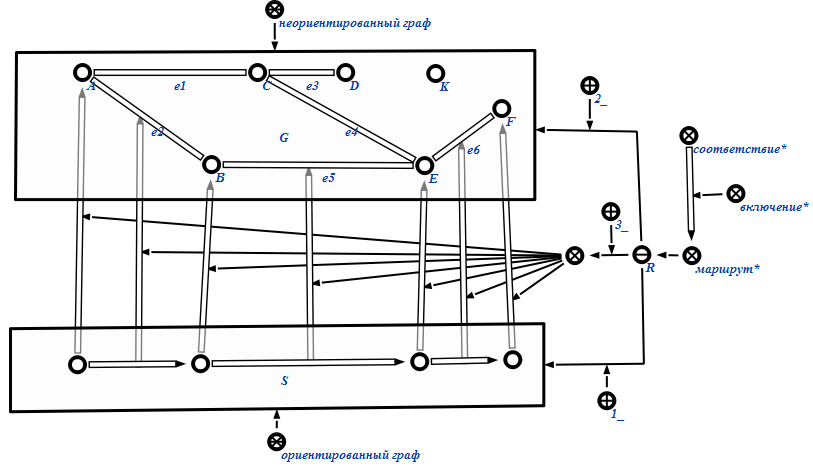
\includegraphics[scale=0.6]{2/Route_as_correspondence_Final}
  \caption{Окончательный вариант представления маршрута \idtf{R}, как
    соответствия между графом \idtf{S} и графом \idtf{G}}
  \label{fig:Route_as_correspondence_Final}
\end{figure}

Попробуйте представить при помощи найденного нами способа
(рис.~\ref{fig:Route_as_correspondence_Final}) маршрут, в котором есть
повторяющиеся вершина и/или ребра. Я думаю, что теперь с этим у вас не
возникнет проблем. Подводя к концу разговор о способе представления
маршрутов в графе, введем относительные понятия (бинарные
ориентированные отношения) \idtf{цепь*} и \idtf{путь*}, которые
связаны с отношением \idtf{маршрут*} так, как показано на
рис.~\ref{fig:Relations_Trail_and_Path}.

\begin{figure}[h!]
  \centering
  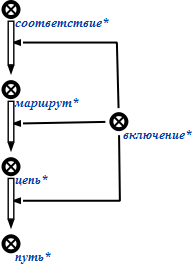
\includegraphics[scale=0.8]{2/Relations_Trail_and_Path}
  \caption{Связь отношений \idtf{цепь*} и \idtf{путь*} с отношением
    \idtf{маршрут*}}
  \label{fig:Relations_Trail_and_Path}
\end{figure}

Тогда один из минимальных путей \idtf{R} (\idtf{A}, \idtfm{$e_2$},
\idtf{B}, \idtfm{$e_5$}, \idtf{E}, \idtfm{$e_6$}, \idtf{F}) в графе
\idtf{G} между вершинами \idtf{A} и \idtf{F} будет представляться в
SC-коде так, как показано на рис.~\ref{fig:Path_Final}. Правда,
несильно отличается от рис.~\ref{fig:Route_as_correspondence_Final}?

\begin{figure}[h!]
  \centering
  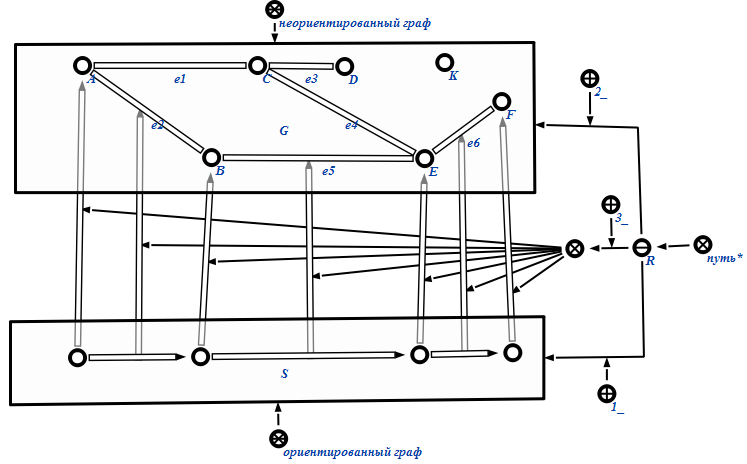
\includegraphics[scale=0.6]{2/Path_Final}
  \caption{Один из минимальных путей \idtf{R} между вершинами \idtf{А}
    и \idtf{F} графа \idtf{G}}
  \label{fig:Path_Final}
\end{figure}

На этом мы заканчиваем разговор о минимальном пути и переходим к
разговору о том, как можно обобщить представление различных видов
графов в SC-коде.

\section{Обобщение различных видов графов с использованием понятия
  графовой структуры}
\label{sec:Onto_graph_struct}

В предыдущем разделе, когда мы искали способ представления
минимального пути в SC-коде, то сосредоточились на представлении
наиболее общего понятия по отношению к понятию путь, а именно –
маршрута. Таким образом, определившись с кодированием понятия
\idtf{маршрут*}, мы определились и с кодированием понятия
\idtf{путь*}. А вот, когда мы разбирались с неориентированными и
ориентированными графами, то рассматривали только то, что необходимо
для решения нашей задачи, игнорируя более общие случаи. Теперь пришло
время посмотреть на задачу представления графов в SC-коде более
широко. Для этого мы обратимся к базе знаний по теории графов из
проекта \ostisgtlink. Неполная иерархия различных типов графов из этой
базы знаний изображена на рис.~\ref{fig:Hierarchy_of_graphs_types}. Я
думаю, что вы уже заметили узлы ориентированный граф и
неориентированный граф. Однако они составляют только <<низ>> иерархии,
так как определены на основе более общих понятий. А начнем
рассматривать иерархию с <<верха>>, а именно, с понятия \idtf{графовая
  структура}.

\begin{figure}[h!]
  \centering
  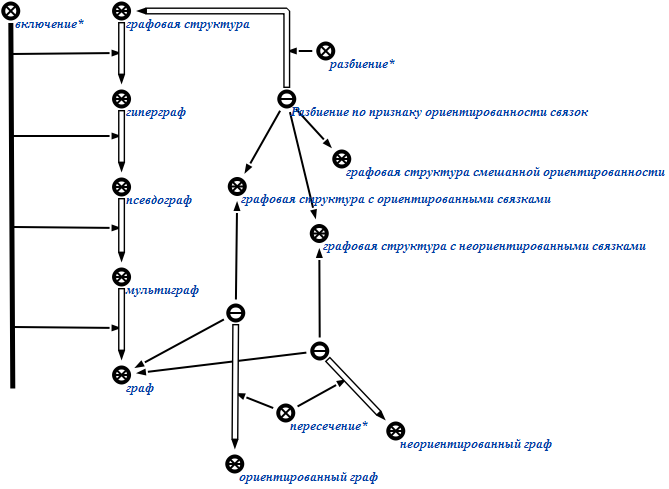
\includegraphics[scale=0.95]{2/Hierarchy_of_graphs_types}
  \caption{Иерархия различных типов графовых структур (Это неполная
    иерархия из \ostisgtlink)}
  \label{fig:Hierarchy_of_graphs_types}
\end{figure}

Экземпляр понятия \idtf{графовая структура} – это такая одноуровневая
реляционная структура, которая содержит объекты с ролью
\idtf{вершина_}, а связки между этими объектами - с ролью
\idtf{связка_}. Вроде бы по определению \idtf{графовая структура}
несильно отличается от \idtf{неориентированного графа}. Взяли просто и
заменили ролевое отношение \idtf{ребро_} на \idtf{связка_}. И вот тут
есть один нюанс. На элементы с ролью \idtf{связка_} \idtf{графовой
  структуры} не накладывается ограничений, как на элементы с ролью
\idtf{ребро_} \idtf{неориентированного графа}, а именно:

\begin{itemize}
\item они могут быть любой арности, а не только бинарными;
\item они могут быть как ориентированными, так и неориентированными;
\item их компонентами могут быть не только вершины, но и другие связки
  (т.е. разрешены связки, <<выходящие>> из связок, и связки, входящие
  в другие связки).
\end{itemize}

На рис.~\ref{fig:Graph_structure_example} приведен пример графовой
структуры \idtfm{$G_s$}, в которой четыре вершины и три связки. Я хочу
отметить, что графовая структура вполне может включать элементы с
ролью \idtf{ребро_}. Просто \idtf{связка_} более общее понятие, чем
\idtf{ребро_}. Чтобы лучше увидеть связь между этими ролевыми
отношениями, рассмотрите
рис.~\ref{fig:Hierarchy_of_elements_roles_in_graph_structure}, на
котором изображена иерархия ролевых отношений элементов графовой
структуры из базы знаний по теории графов. А после того, как
закончите, мы перейдем к краткому описанию абсолютных понятий
\idtf{гиперграф}, \idtf{псевдограф}, \idtf{мультиграф} и \idtf{граф}.

\begin{figure}[h!]
  \centering
  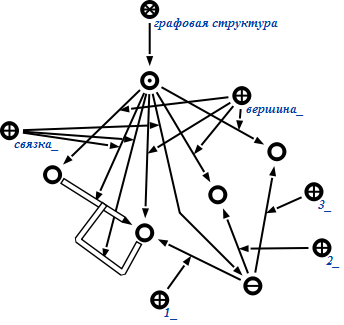
\includegraphics{2/concept/Graph_structure}
  \caption{Пример графовой структуры \idtfm{$G_s$}}
  \label{fig:Graph_structure_example}
\end{figure}
 
\begin{figure}[h!]
  \centering
  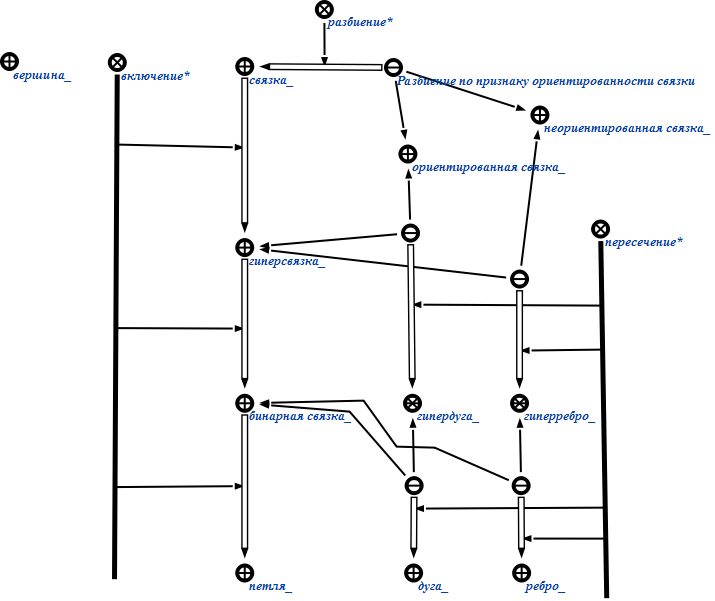
\includegraphics[scale=0.95]{2/Hierarchy_of_elements_roles_in_graph_structure}
  \caption{Иерархия ролей элементов графовой структуры (Это неполная
    иерархия из \ostisgtlink)}
  \label{fig:Hierarchy_of_elements_roles_in_graph_structure}
\end{figure}

Экземпляр понятия \idtf{гиперграф}
(см. рис.~\ref{fig:Hierarchy_of_graphs_types}) – это такая графовая
структура, в которой элемент с ролью \idtf{связка_} может иметь в
качестве своих компонентов только элемент с ролью \idtf{вершина_} этой
графовой структуры.  На арность связок никакого ограничения не
накладывается. Для указания связки введены ролевые отношения
\idtf{гиперсвязка_}, \idtf{гипердуга_}, \idtf{гиперребро_}
(рис.~\ref{fig:Hierarchy_of_elements_roles_in_graph_structure}). Обратите
внимание на то, что на
рис.~\ref{fig:Hierarchy_of_elements_roles_in_graph_structure}
\idtf{гипердуга_} определена как пересечение понятий \idtf{гиперсвязка_}
и {ориентированная связка}. Аналогично дела обстоят с понятием
\idtf{гиперребро_}. Пожалуйста, обдумайте самостоятельно такой способ
введения новых понятий.

Экземпляр понятия \idtf{псевдограф}
(см. рис.~\ref{fig:Hierarchy_of_graphs_types}) – это такой гиперграф,
в котором гиперсвязка может иметь только два компонента.  Для указания
связки введены ролевые отношения \idtf{бинарная связка_}, \idtf{петля_},
\idtf{дуга_}, \idtf{ребро_}
(рис.~\ref{fig:Hierarchy_of_elements_roles_in_graph_structure}). Петлей
называется бинарная связка, у которой оба компонента одинаковы.

Экземпляр понятия \idtf{мультиграф}
(см. рис.~\ref{fig:Hierarchy_of_graphs_types}) – это такой псевдограф,
в котором не может быть петель.
 
Экземпляр понятия \idtf{граф}
(см. рис.~\ref{fig:Hierarchy_of_graphs_types}) – это такой мультиграф,
в котором не может быть кратных связок, т.е. связок у которых первый и
второй компоненты совпадают.

А теперь самостоятельно на основе
рис.~\ref{fig:Hierarchy_of_graphs_types} рассмотрите то, как
определены уже знакомые вам понятия \idtf{ориентированный граф} и
\idtf{неориентированный граф}. 

\newpage

\section{Пример выполнения}
\label{sec:Onto_example}

\subsection{Список понятий}
\label{sec:Onto_ex_concepts}

\begin{itemize}
\item Графовая структура (абсолютное понятие) - это такая
  одноуровневая реляционная структура, объекты которой могут играть
  роль либо вершины, либо связки:
  \begin{itemize}
  \item Вершина (относительное понятие, ролевое отношение);
  \item Связка (относительное понятие, ролевое отношение).
  \end{itemize}

  \begin{figure}[h!]
    \centering
    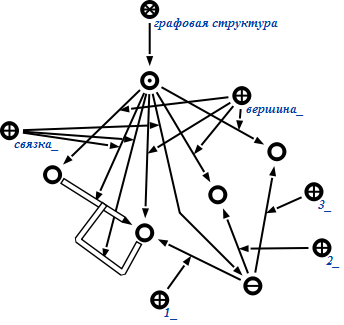
\includegraphics[scale=0.8]{2/concept/Graph_structure}
    \label{fig:Concept_Graph_structure}
  \end{figure}

\newpage

\item Графовая структура с ориентированными связками (абсолютное
  понятие)
  \begin{itemize}
  \item Ориентированная связка (относительное понятие, ролевое
    отношение) – связка, которая задается ориентированным множеством.
  \end{itemize}

  \begin{figure}[h!]
    \centering
    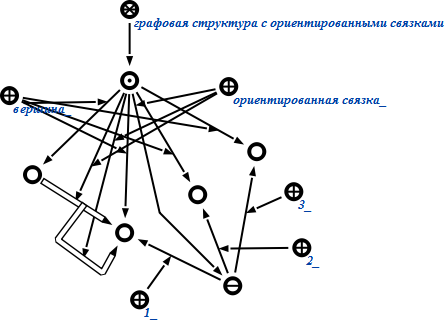
\includegraphics[scale=0.8]{2/concept/Directed_graph_structure}
    \label{fig:Concept_Directed_graph_structure}
  \end{figure}

\newpage

\item Графовая структура с неориентированными связками (абсолютное
  понятие)
  \begin{itemize}
  \item Неориентированная связка (относительное понятие, ролевое
    отношение) – связка, которая задается неориентированным
    множеством.
  \end{itemize}

  \begin{figure}[h!]
    \centering
    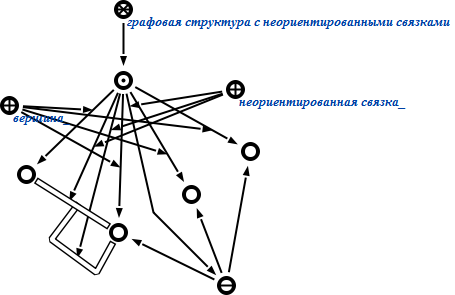
\includegraphics[scale=0.8]{2/concept/Undirected_graph_structure}
    \label{fig:Concept_Undirected_graph_structure}
  \end{figure}

\newpage

\item Гиперграф (абсолютное понятие) – это такая графовая структура, в
  которой связки могут связывать только вершины:
  \begin{itemize}
  \item Гиперсвязка (относительное понятие, ролевое отношение);
  \item Гипердуга (относительное понятие, ролевое отношение) –
    ориентированная гиперсвязка;
  \item Гиперребро (относительное понятие, ролевое отношение) –
    неориентированная гиперсвязка.
  \end{itemize}

  \begin{figure}[h!]
    \centering
    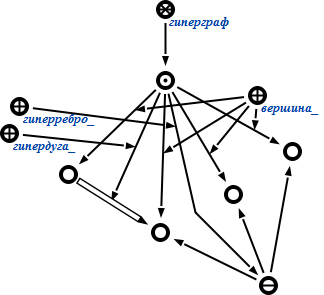
\includegraphics[scale=0.8]{2/concept/Hypergraph}
    \label{fig:Concept_Hypergraph}
  \end{figure}

\newpage

\item Псевдограф (абсолютное понятие) – это такой гиперграф, в котором
  все связки должны быть бинарными.
  \begin{itemize}
  \item Бинарная связка (относительное понятие, ролевое отношение)
    – гиперсвязка арности 2; 
  \item Ребро (относительное понятие, ролевое
    отношение) – неориентированная гиперсвязка;
  \item Дуга (относительное понятие, ролевое отношение) –
    ориентированная гиперсвязка;
  \item Петля (относительное понятие, ролевое отношение) – бинарная
    связка, у которой первый и второй компоненты совпадают.
  \end{itemize}

  \begin{figure}[h!]
    \centering
    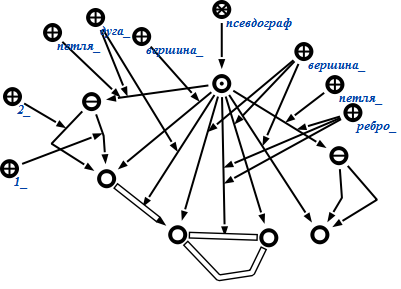
\includegraphics[scale=0.8]{2/concept/Pseudograph}
    \label{fig:Concept_Pseudograph}
  \end{figure}

\newpage

\item Мультиграф (абсолютное понятие) – это такой псевдограф, в
  котором не может быть петель.

  \begin{figure}[h!]
    \centering
    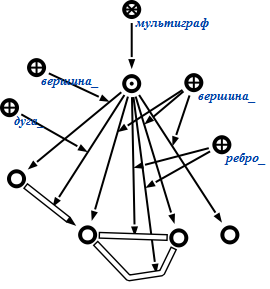
\includegraphics[scale=0.8]{2/concept/Multigraph}
    \label{fig:Concept_Multigraph}
  \end{figure}

\newpage
 
\item Граф (абсолютное понятие) – это такой мультиграф, в котором не
  может быть кратных связок, т.е. связок у которых первый и второй
  компоненты совпадают.

  \begin{figure}[h!]
    \centering
    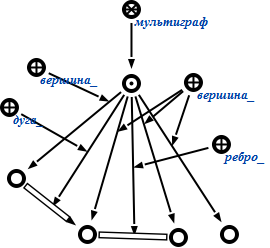
\includegraphics[scale=0.8]{2/concept/Graph}
    \label{fig:Concept_Graph}
  \end{figure}

\newpage
 
\item Неориентированный граф (абсолютное понятие) – это такой граф, в
  котором все связки являются ребрами:

  \begin{figure}[h!]
    \centering
    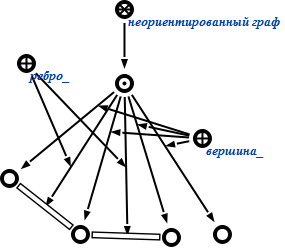
\includegraphics[scale=0.8]{2/concept/Undirected_graph}
    \label{fig:Concept_Undirected_graph}
  \end{figure}

\newpage
 
\item Ориентированный граф (абсолютное понятие) - это такой граф, в
  котором все связки являются дугами:

  \begin{figure}[h!]
    \centering
    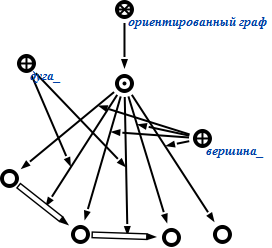
\includegraphics[scale=0.8]{2/concept/Directed_graph}
    \label{fig:Concept_Directed_graph}
  \end{figure}

\newpage
 
\item Маршрут (относительное понятие, бинарное ориентированное
  отношение) – это чередующаяся последовательность вершин и
  гиперсвязок в гиперграфе, которая начинается и кончается вершиной, и
  каждая гиперсвязка последовательности инцидентна двум вершинам, одна
  из которых непосредственно предшествует ей, а другая непосредственно
  следует за ней. В примере ниже показан маршрут \idtf{A},
  \idtf{CON1}, \idtf{C}, \idtf{CON2}, \idtf{D}, \idtf{CON3}, \idtf{B},
  \idtf{CON1}, \idtf{A} в гиперграфе. Обратите внимание, что графы в
  примере приведены в сокращенной форме, что \idtf{CON1} – это
  тернарная неориентированная связка (гиперсвязка), а \idtf{CON2} и
  \idtf{CON3} – бинарные связки (гиперсвязки).

  \begin{figure}[h!]
    \centering
    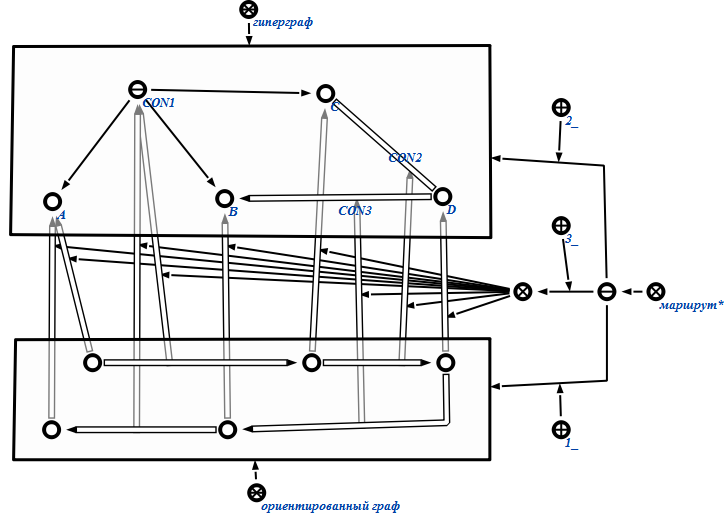
\includegraphics[scale=0.8]{2/concept/Route}
    \label{fig:Concept_Route}
  \end{figure}

\newpage
 
\item Цепь (относительное понятие, бинарное ориентированное отношение)
  – это маршрут, все гиперсвязки которого различны. В примере ниже
  показана цепь \idtf{A}, \idtf{CON1}, \idtf{C}, \idtf{CON2},
  \idtf{D}, \idtf{CON3}, \idtf{B}, \idtf{CON1}, \idtf{A} в гиперграфе.

  \begin{figure}[h!]
    \centering
    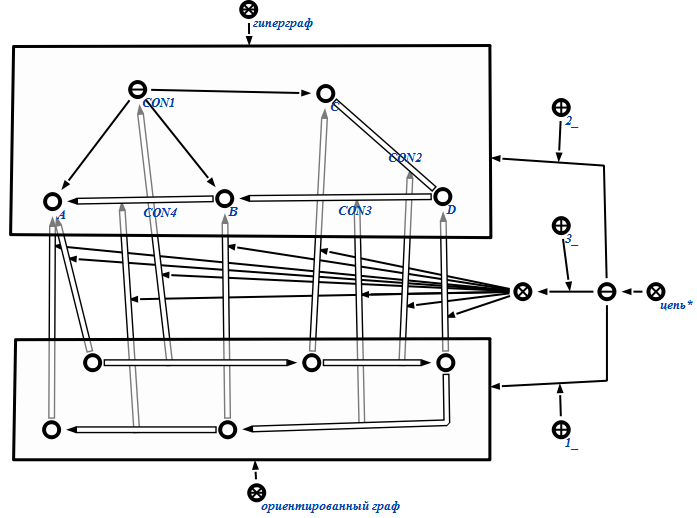
\includegraphics[scale=0.8]{2/concept/Trail}
    \label{fig:Concept_Trail}
  \end{figure}

\newpage
 
\item Простая цепь, путь (относительное понятие, бинарное
  ориентированное отношение) – это цепь, в которой все вершины
  различны. В примере ниже показан путь \idtf{A}, \idtf{CON1},
  \idtf{C}, \idtf{CON2}, \idtf{D}, \idtf{CON3}, \idtf{B} в гиперграфе.

  \begin{figure}[h!]
    \centering
    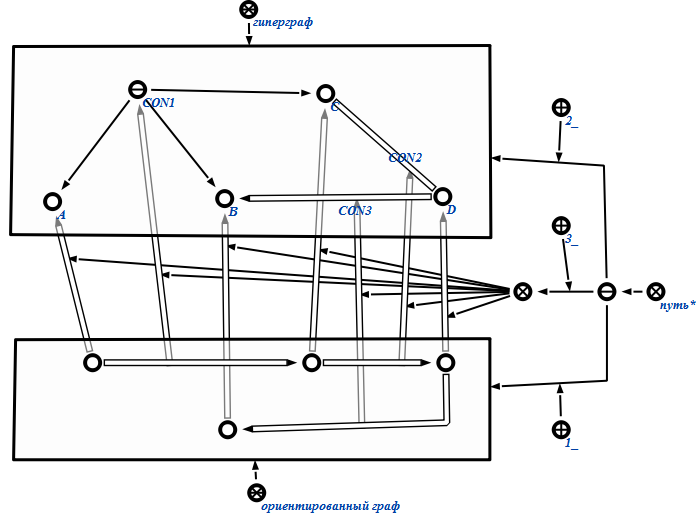
\includegraphics[scale=0.8]{2/concept/Path}
    \label{fig:Concept_Path}
  \end{figure}

\end{itemize}

\newpage

\subsection{Тестовые примеры}
\label{sec:Onto_ex_tests}

Во всех тестах графы будет приведены в сокращенной форме со скрытыми
ролями элементов графа.

\newcounter{ontotests}

\newenvironment{test}
{
  \addtocounter{ontotests}{1}

  \newpage
  \subsubsection{Тест \arabic{ontotests}}
}
{
}

\newcommand{\testnum}{\arabic{ontotests}}

\newcommand{\testin}[2][1.0]
{
  \begin{figure}[h!]
    \centering
    \includegraphics[scale=#1]{2/test/#2_In}
    \label{fig:Test#2_In}
  \end{figure}
}

\newcommand{\testout}[2][1.0]
{
  \begin{figure}[h!]
    \centering
    \includegraphics[scale=#1]{2/test/#2_Out}
    \label{fig:Test#2_Out}
  \end{figure}
}

\begin{test}
  \textbf{Вход:} Необходимо найти минимальный путь между вершинами $A$
  и $C$.

  \testin\testnum

  \textbf{Выход:} Будет найден единственный минимальный путь $A$,
  $E1$, $B$, $E2$, $C$:

  \testout\testnum
\end{test}

\begin{test}
  \textbf{Вход:} Необходимо найти минимальный путь между вершинами $A$
  и $F$.

  \testin[0.8]\testnum

  \textbf{Выход:} Будет найден один из двух минимальный путь $A$,
  $E2$, $B$, $E3$, $D$, $E5$, $F$:

  \testout[0.8]\testnum
\end{test}

\begin{test}
  \textbf{Вход:} Необходимо найти минимальный путь между вершинами $A$
  и $K$.

  \testin\testnum

  \textbf{Выход:} Минимального пути между вершинами $A$ и $K$ не
  существует. Программа должна вернуть ошибку вызывающему контексту.
\end{test}

\begin{test}
  \textbf{Вход:} Необходимо найти минимальный путь между вершинами
  $V5$ и $V11$.

  \testin[0.8]\testnum

  \textbf{Выход:} Будет найден один из двух минимальный путь $V5$,
  $E8$, $V7$, $E9$, $V6$, $E11$, $V9$, $E15$, $V11$:

  \testout[0.8]\testnum
\end{test}

\begin{test}
  \textbf{Вход:} Необходимо найти минимальный путь между вершинами
  $V1$ и $V9$.

  \testin[0.8]\testnum

  \textbf{Выход:} Минимального пути между вершинами $V1$ и $V9$ не
  существует. Программа должна вернуть ошибку вызывающему контексту.
\end{test}

%%% Local Variables: 
%%% mode: latex
%%% TeX-master: "main"
%%% End: 

\chapter{Демонстрация работы программы решения теоретико-графовой
  задачи в семантической памяти}

\section{Задание}

На этом этапе выполнения расчетной работы вам необходимо будет
продемонстрировать пошаговое выполнение алгоритма в sc-памяти. Сам
алгоритм и структуры данных для него вы уже исследовали на предыдущих
этапах расчетной работы, а сейчас надо будет продемонстрировать
графодинамику выполнения алгоритма. Это значит, что вся информация,
необходимая для работы вашего алгоритма, должна храниться в sc-памяти
и там же и обрабатываться. В качестве примера <<неудобства>>, которое
вам может принести такое требование, я могу привести невозможность
использования привычной матрицы смежности/инцидентности.  Поэтому для
прохождения этого этапа вам придется взглянуть на алгоритм, решающий
выбранную задачу, под другим углом.

\section{Волновой алгоритм поиска одного из минимальных путей в
  неориентированном графе}

\subsection{Описание алгоритма}
\label{sec:-Algo_desc}

Алгоритм поиска одного из минимальных путей в неориентированном графе
является волновым и основан на понятии волны. В рамках этого алгоритма
волной называется множество вершин, каждая из которых является в
обрабатываемом графе смежной хотя бы одной вершине из предыдущей
волны. Волна, для которой нет предыдущей волны, называется начальной и
состоит из вершины, от которой начинается поиск минимального
пути. Волна, включающая конечную вершину пути, называется
конечной. Таким образом, наш алгоритм можно задать следующим перечнем
шагов:

\begin{enumerate}
\item Добавить все вершины графа, кроме начальной вершины пути, во
  множество непроверенных вершин.
\item Создать новую волну и добавить в нее начальную вершину пути.
\item Начальная волна – это новая волна. Новой волной будем называть
  последнюю созданную волну.
\item Сформировать следующую волну для новой волны. В нее попадет та
  вершина, которая является смежной вершине из новой волны и
  присутствует во множестве непроверенных вершин. Если вершина попала
  в формируемую волну, то ее надо исключить из множества непроверенных
  вершин. Созданную волну установить как следующую для новой волны, и
  после этого созданную волну считать новой волной.
\item Если новая волна пуста, то между вершинами не существует
  пути. Завершить алгоритм.
\item Если в текущей волне есть конечная вершина, то перейти к пункту
  7, иначе к пункту 4.
\item Сформировать один из минимальных путей, проходя в обратном
  порядке по списку волн. Завершить алгоритм.
\end{enumerate}

\subsection{Пример выполнения алгоритма в sc-памяти}

\subsubsection{Соглашения по демонстрации}

Перед демонстрацией выполнения алгоритма в sc-памяти нам необходимо
установить некоторые соглашения по формирование SCg-рисунков.

При записи графов я буду использовать сокращенную форму - атрибуты для
вершин и связок не приводятся, однако вы должны помнить, что
сокращенная форма используется только для наглядности.

В качестве программных переменных, которые используются в ходе работы
алгоритма, я буду использовать sc-переменные. Для указания значения
sc-переменной используется отношение \rel{значение}.  На рисунке 3.1
задано значение для sc-переменной \vidtf{beg\_vertex}.

\begin{figure}[h!]
  \centering
  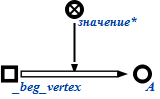
\includegraphics{images/3/Value_sc_var}
  \caption{Пример указания значения sc-переменной \vidtf{beg\_vertex}}
  \label{fig:Value_sc_var}
\end{figure}

Однако я буду сокращать способ, показанный на
рис.~\ref{fig:Value_sc_var}, опуская знак отношения
\rel{значение}. Таким образом, будет использована форма, показанная на
рис.~\ref{fig:Short_value_sc_var}. Имейте в виду, что полученная
sc-конструкция не является корректной в семантическом смысле, но в
данном разделе использование именно такой формы позволит сделать
рисунки более понятными.

\begin{figure}[h!]
  \centering
  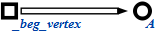
\includegraphics{images/3/Short_value_sc_var}
  \caption{Пример сокращенного указания значения sc-переменной
    \vidtf{beg\_vertex}}
  \label{fig:Short_value_sc_var}
\end{figure}

Последнее, о чем мы договоримся, будет использование цветов с целью
явного выделения изменений, произошедших с sc-конструкцией. Для этого
я буду использовать следующий перечень цветов:

\begin{itemize}
\item \textcolor{magenta}{фиолетовым} цветом будут выделяться sc-переменные, значение
  которых изменилось;
\item \textcolor{green}{зеленым} цветом будут выделяться созданные sc-элементы;
\item \textcolor{blue}{синим} цветом будут выделяться измененные sc-элементы (например,
  sc-множества, в которые был включен или из которых был исключен
  элемент).
\end{itemize}

Пришло время посмотреть, как же работает наш алгоритм в sc-памяти.

\subsubsection{Демонстрация алгоритма}

Выполнение алгоритма я продемонстрирую через состояния sc-памяти на
каждом элементарном этапе решения задачи. Для всех элементарных
этапов, для которых это возможно, в конце их краткого описания в
скобках будет указан соответствующий номер шага алгоритма из раздела
\ref{sec:-Algo_desc}.

\newenvironment{algostep}[3]
{
  \newpage
  \emph{\textbf{#1}}

  \begin{figure}[h!]
    \centering
    \includegraphics[scale=#3]{images/3/#2}
    \label{fig:#2}
  \end{figure}
}


\begin{algostep}{Задание входного графа, начальной и конечной вершины
    пути для работы алгоритма}{S1_Input_graph}{0.8}
  
  Переменные изменятся следующим образом:

  \begin{itemize}
  \item \vidtf{graph} получит в качестве значения sc-узел
    неориентированного графа;
  \item \vidtf{beg\_vertex} получит в качестве
    значения вершину А, которая будет начальной для поиска минимального
    пути;
  \item \vidtf{end\_vertex} получит в качестве значение вершину $F$,
    которая будет конечной для поиска минимального пути.  Таким образом,
    из состояния sc-памяти на этом шаге вам должно быть ясно, что будет
    производиться поиск минимального пути между вершинами $A$ и $F$.
  \end{itemize}
\end{algostep}


\begin{algostep}{Создание множества непроверенных вершин (Шаг
    1)}{S2_Create_unchecked_vertexes_set}{0.8}

  Переменная \vidtf{not\_checked\_vertexes} получит в качестве значения
  множество непроверенных вершин обрабатываемого графа (в это множество
  не включена начальная вершина пути $A$).
\end{algostep}


\begin{algostep}{Создание волны, включающей начальную вершину A (Шаги
    2, 3)}{S3_Create_1st_wave}{0.8}

  На этом этапе программа создает первую волну из списка волн. Первая
  волна содержит только начальную вершину пути $A$. Переменная
  \vidtf{new\_wave} получает в качестве значения созданную волну, и в
  будущем будет всегда указывать на вновь созданную волну.

  Переменная \vidtf{waves\_list\_head} указывает на начальный элемент
  списка волн, а переменная \vidtf{waves\_list\_tail} сейчас и в
  последующих шагах – на концевой элемент списка волн.
\end{algostep}


\begin{algostep}{Создание волны, включающей вершины B и С (Шаг
    4)}{S4_Create_next_wave}{0.8}
  
  Для вершин из предыдущей волны являются смежными и входящими во
  множество проверенных вершин только вершины $B$ и $С$. Из них
  формируем новую волну. Обратите внимание на то, что эти вершины
  исключаются из множества непроверенных вершин (см. значение
  переменной \vidtf{not\_checked\_vertexes}).

  Переменная \vidtf{waves\_list\_tail} получает в качестве значения
  созданный элемент списка, а переменная \vidtf{new\_wave} – созданную
  волну.
\end{algostep}


\begin{algostep}{Создание волны, включающей вершину D (Шаг
    4)}{S5_Create_next_wave}{0.8}

  Для вершин из предыдущей волны является смежной и входящей во
  множество проверенных вершин только вершина $D$. Из нее формируем
  новую волну. Обратите внимание на то, что эта вершина исключается из
  множества непроверенных вершин (см. значение переменной
  \vidtf{not\_checked\_vertexes}).

  Переменная \vidtf{waves\_list\_tail} получает в качестве значения
  созданный элемент списка, а переменная \vidtf{new\_wave} – созданную
  волну.
\end{algostep}


\begin{algostep}{Создание волны, включающей вершину F (Шаги 4, 5,
    6)}{S6_Create_last_wave}{0.8}

  Для вершины из предыдущей волны является смежной и входящей во
  множество проверенных вершин только вершина $F$. Из нее формируем
  новую волну. Обратите внимание на то, что эта вершина исключается из
  множества непроверенных вершин (см. значение переменной
  \vidtf{not\_checked\_vertexes}).

  Переменная \vidtf{waves\_list\_tail} получает в качестве значения
  созданный элемент списка, а переменная \vidtf{new\_wave} – созданную
  волну.

  Так как эта волна содержит конечную вершину пути $F$, то на
  следующих этапах мы перейдем к генерации одного из найденных
  минимальных путей.
\end{algostep}


\begin{algostep}{Удаление множества непроверенных
    вершин}{S7_Erase_unchecked_vertexes_set}{0.8}
 
  Подчистим память, удалив множество непроверенных вершин (значение
  переменной \vidtf{not\_checked\_vertexes}), так как оно нам уже не
  надо.
\end{algostep}


\begin{algostep}{Создание связки отношения \rel{путь} (Шаг
    8)}{S8_Create_route_tuple}{0.7}
 
  Начинаем генерацию одного из найденных минимальных путей.

  Создадим связку отношения \rel{путь} и установим ее в качестве
  значения переменной \vidtf{route}. Переменная \vidtf{route\_struct}
  получит в качестве значения ориентированный граф структуры пути, а
  переменная \vidtf{route\_visit} – отношения посещения.
\end{algostep}


\begin{algostep}{Добавление в структуру пути посещения начальной и
    конечной вершины генерируемого пути (Шаг
    8)}{S9_Add_begin_and_end_vertexes_visit_to_route_tuple}{0.7}
 
  Добавим в структуру генерируемого пути посещения начальной вершины
  $A$ и конечной вершины $F$. Созданные посещения получат в качестве
  значения переменные \vidtf{beg\_vertex\_visit} и
  \vidtf{end\_vertex\_visit}.
\end{algostep}


\begin{algostep}{Установка переменных для 1-ой итерации цикла генерации
    структуры пути (Шаг 8)}{S10_Step_building_route_structure}{0.7}
  
  Структура пути строится, начиная с конечной вершины пути $F$.

  На этом этапе переменная \vidtf{curr\_vertex} получит в качестве
  значения текущую обрабатываемую вершину, переменная \vidtf{list\_it}
  – текущий обрабатываемый элемент списка волн, переменная
  \vidtf{curr\_wave} – текущую обрабатываемую волну.
\end{algostep}

 
\begin{algostep}{Создание посещения вершины на 1-ой итерации цикла
    генерации структуры пути (Шаг
    8)}{S11_Step_building_route_structure_add_visits}{0.7}
 
  Создадим посещение для одной из вершин из волны \vidtf{curr\_wave},
  которая является смежной вершине из переменной
  \vidtf{curr\_vertex}. Для связывающего их ребра тоже создадим
  посещение.
\end{algostep}  


\begin{algostep}{Переход ко 2-ой итерации цикла генерации структуры
    пути (Шаг 8)}{S12_Step_building_route_structure}{0.7}
 
  На этом этапе переменная \vidtf{curr\_vertex} получит в качестве
  значения вершину, для которой было создано посещение на предыдущей
  итерации. Переменная \vidtf{list\_it} – предшествующей элемент
  списка волн для значения переменной \vidtf{curr\_wave} на предыдущем
  этапе. Переменная \vidtf{curr\_wave} – обрабатываемую волну для
  элемента списка из установленного значения \vidtf{list\_it}.
\end{algostep}


\begin{algostep}{Создание посещения вершины на 2-ой итерации цикла
    генерации структуры пути (Шаг
    8)}{S13_Step_building_route_structure_add_visits}{0.7}

  Создадим посещение для одной из вершин из волны \vidtf{curr\_wave},
  которая является смежной вершине из переменной
  \vidtf{curr\_vertex}. На эту роль была выбрана вершина $С$. Для
  ребра, связывающего две вершины, тоже создадим посещение.
\end{algostep}


\begin{algostep}{Переход к 3-ей итерации цикла генерации структуры пути
    (Шаг 8)}{S14_Step_building_route_structure}{0.7}
 
  На этом этапе переменная \vidtf{curr\_vertex} получит в качестве
  значения вершину, для которой было создано посещение на предыдущей
  итерации. Переменная \vidtf{list\_it} – предшествующей элемент
  списка волн для значения переменной \vidtf{curr\_wave} на предыдущем
  этапе. Переменная \vidtf{curr\_wave} – обрабатываемую волну для
  элемента списка из установленного значения \vidtf{list\_it}.
\end{algostep}


\begin{algostep}{Создание посещения вершины на 3-ей итерации цикла
    генерации структуры пути (Шаг
    8)}{S15_Step_building_route_structure_add_visits}{0.7}
 
  Так как для вершины $A$ уже создано посещение, то делать это
  повторно алгоритм не будет. А вот посещение ребра между вершинами
  $A$ и $С$ необходимо создать.

  Структура пути создано, поэтому завершаем цикл и переходим к очистке
  sc-памяти от уже ненужных sc-конструкций.
\end{algostep}

\begin{algostep}{Удаление списка волн}{S16_Erase_waves_list}{0.7}
 
  Удалим список волн. Переменные \vidtf{list\_it},
  \vidtf{waves\_list\_head}, \vidtf{curr\_wave},
  \vidtf{waves\_list\_tail} окажутся без значений.
\end{algostep}


\begin{algostep}{Результат работы алгоритма}{S17_Result}{0.7}
 
  На данном этапе продемонстрирован результат работы алгоритма,
  значение переменной \vidtf{route} будет возвращено в вызывающий
  контекст.
\end{algostep}


%%% Local Variables: 
%%% mode: latex
%%% TeX-master: "main"
%%% End: 


\end{document}


